\documentclass[12pt, a4paper, oneside]{report}

%% COMMANDS FOR THE TITLE PAGE CONTENT

% SW Author name (capitalized in its regular way)
\newcommand{\authorname}{Sean Allen Siegfreid R. Bugarin}

% SW Report Title (cannot exceed three lines)
% WORKING TITLE. The author chooses the final title.
\newcommand{\thetitle}{GroundLoop: A Self-Checking Agentic RAG System with Evaluation-Guided Recovery}

% Date of submission with normal capitalization.
% Use the format January 29, 2027.
% Fall 2026 final submission deadline per the Office of Signature Work guideline.
\newcommand{\submissiondate}{November 2, 2026}

% Mentor: First Name Last Name (normal capitalization)
\newcommand{\mentor}{Bing Luo}
% Mentor's Academic Unit (no abbreviations)
\newcommand{\mentoracademicunit}{Division of Natural and Applied Sciences}

% No co-mentor.
\newcommand{\comentor}{}

% Co-mentor's Academic Unit (no abbreviations)
% If the co-mentor is empty, the following will be ignored.
\newcommand{\comentoracademicunit}{}


%% PACKAGES

\usepackage[a4paper, margin=1in]{geometry}
\usepackage{parskip}

\usepackage{amsmath, amsthm}

% Office of Signature Work formatting: Times New Roman (or Garamond, Cambria,
% Arial) at 12 pt, double spaced, 1 inch margins. newtx supplies Times for
% text and math; amssymb is omitted because newtxmath provides its symbols.
\usepackage[T1]{fontenc}
\usepackage{newtxtext, newtxmath}
\renewcommand{\sfdefault}{\rmdefault}
\usepackage{graphicx}
\usepackage{xcolor}
\usepackage{longtable, booktabs, array}

\usepackage{upquote}
\usepackage{microtype}

\usepackage{titlesec}
\titleformat{\chapter}[display]
  {\sffamily\bfseries\huge}
  {\Large\chaptertitlename\ \thechapter}
  {2ex}
  {\titlerule\vspace{1ex}\filright\MakeUppercase}
  [\vspace{1ex}\titlerule]
\titleformat{\section}{\normalfont\sffamily\Large\bfseries}{\thesection}{1em}{}
\titleformat{\subsection}{\normalfont\sffamily\large\bfseries}{\thesubsection}{1em}{}
\titleformat{\subsubsection}{\normalfont\sffamily\normalsize\bfseries}{\thesubsubsection}{1em}{}

\usepackage[style=numeric-comp, url=false]{biblatex}
\addbibresource{references.bib}

% Orange text inside the \instructions command must not appear
% in the final version of your report. You can either delete it
% from your document, or redefine the command \instructions, by
% commenting out the definition here...
\newcommand{\instructions}[1]{}
\newcommand{\authornote}[1]{}

\newcommand{\code}[1]{\texttt{\detokenize{#1}}}

\usepackage{tikz}
\usetikzlibrary{arrows.meta, positioning}

\usepackage[allcolors=blue, colorlinks=true]{hyperref}
\usepackage{xurl}
\usepackage{bookmark}

\urlstyle{same}

\usepackage{calc}
\usepackage{xifthen}
\usepackage{etoolbox}

\usepackage{setspace}

\begin{document}

\thispagestyle{empty}

% About Majors at DKU
Background:  Duke Kunshan University (DKU) is an interdisciplinary institution that grants dual undergraduate degrees, an MOE Chinese degree and a degree from Duke University in Durham, United States. The principal structure of DKU majors is robustly interdisciplinary. No student confines their study to a single discipline (for example, biology or economics). Instead, all students engage in broad inquiry related to a subject or question (for example, political economy or global health) and take a wide variety of courses related to that area (for example, in public policy, history, ethics, or economics). As a result, our graduates are prepared to engage in a wide variety of inquiries using multiple methodologies to address complex issues that require interdisciplinary approaches.  

This has implications for our vision and expectations of undergraduate theses and design projects, which reflect this broad interdisciplinary training. At DKU, every student completes a two-year project known as signature work which consists of multiple interconnected parts including thematic courses, experiential learning, capstones, and a final product. It seeks to integrate students’ interdisciplinary educational experience and culminates in the creation of a product in a scholarly, creative, or applied nature in lieu of an undergraduate thesis or design required by JED. Because DKU encourages students to cultivate their independence and creativity as one of its institutional student learning outcomes, the student-led signature work projects often reflect students’ own particular interdisciplinary interests and training.  In addition, signature work has an intensive emphasis on problem-solving and skill-development which is much needed for any interdisciplinary inquiry; thus, students’ final products are evidence of transferrable skills that students have acquired and demonstrated through the 2-year program, rather than content knowledge narrowly defined by disciplinary training. 
 
In sum, while the Chinese major declared with any given student might be construed narrowly, the experience of our students is much broader—and intentionally so.  This is a distinctive feature of our curriculum, and this distinctiveness results in broadly interdisciplinary submissions from our graduates’ submitting theses or design projects. We have designed this to prepare our students for a wide variety of graduate programs in China and the West, where interdisciplinary training is a competitive advantage.

%%%%%%%%%%%%%%%%%%%%%%%%%%%%%%%%%%%%%%%%%%%%%%%%%%%%%%%%%%%%%%%%

%% DO NOT CHANGE DIRECTLY THE CONTENTS OF THE TITLE PAGE.
%% TO CUSTOMIZE THE TITLE PAGE CHANGE THE DEFINITIONS OF THE COMMANDS
%% \authorname, \thetitle, \submissiondate
%% \mentor, \mentoracademicunit
%% \comentor, \comentoracademicunit

\begin{titlepage}

\vspace*{\bigskipamount}

\begin{center}
{\sffamily\LARGE\bfseries\MakeUppercase\thetitle\par}

\bigskip

by

\bigskip

{\Large \authorname}

\bigskip

Signature Work Product, in partial fulfillment of the \\
Duke Kunshan University Undergraduate Degree Program

\bigskip

\emph{\submissiondate}

\bigskip

Signature Work Program \\
Duke Kunshan University

\end{center}

\vfill

\textbf{\textsf{APPROVALS}}

\vspace{3em}\hrule\par
Mentor: \mentor, \mentoracademicunit

\ifthenelse{\equal{\comentor}{}}{}{
\vspace{3em}\hrule\par
Co-Mentor: \comentor, \comentoracademicunit
}

\end{titlepage}

%%%%%%%%%%%%%%%%%%%%%%%%%%%%%%%%%%%%%%%%%%%%%%%%%%%%%%%%%%%%%%%%

% Front matter
\clearpage
\pagenumbering{roman}

%%%%%%%%%%%%%%%%%%%%%%%%%%%%%%%%%%%%%%%%%%%%%%%%%%%%%%%%%%%%%%%%

% Only top-level units (chapters) should appear in the TOC
\setcounter{tocdepth}{0} 
\tableofcontents

\doublespacing % τοῖς κείνων ρήμασι πειθόμενοι

%%%%%%%%%%%%%%%%%%%%%%%%%%%%%%%%%%%%%%%%%%%%%%%%%%%%%%%%%%%%%%%%

\chapter*{Abstract}
\addcontentsline{toc}{chapter}{Abstract}

% Abstract in English

GroundLoop is a working application for building question-answering systems
over one's own documents that check their own answers. For each question
it retrieves passages, answers, evaluates the answer with a language-model
judge and deterministic checks, diagnoses the failure, recovers by
rewriting, widening retrieval, regenerating, or abstaining, and verifies
the result. A web console shows every step, and every run is kept as a
trace. The project then asks how far that self-check can be trusted. On
three small collections (88 questions), the loop was compared with a
retrieve-once baseline at 1, 2, and 4 passages and with a plain 8-passage
baseline, three times each. With one passage the loop raised correct
answers from 0.81 to 0.97 on one collection and to 1.00 on the other two,
with one real regression in 27 loop runs. The 8-passage baseline matched it
at under half the cost. The loop's diagnosis matched an offline gold class
for most failures, and its verdict matched gold on 59 of 73 answerable
recoveries, but once it reported a repair after only changing the source
an answer named.

\textbf{Keywords:} GroundLoop; retrieval-augmented generation; agentic
RAG; runtime evaluation; recovery verification.

\vspace{4\bigskipamount}


%%%%%%%%%%%%%%%%%%%%%%%%%%%%%%%%%%%%%%%%%%%%%%%%%%%%%%%%%%%%%%%%

\chapter*{Acknowledgements}
\label{acknowledgements}
\addcontentsline{toc}{chapter}{Acknowledgements}

I thank Bing Luo for mentoring this Signature Work, and Mingxi, a doctoral
student in his group, who guided my research on ChatDKU. That work on
evaluating a campus question-answering system is what led to the question
this project studies. Bing Luo and Mingxi also provided the language-model
API keys used to run the experiments. I also thank Paul Weng, whose summer research
first introduced me to evaluating AI systems.

\newpage

%%%%%%%%%%%%%%%%%%%%%%%%%%%%%%%%%%%%%%%%%%%%%%%%%%%%%%%%%%%%%%%%

% Add captions to your figures for them to appear in the List of Figures.
% Alternatively, comment out the next two lines if there are no tables 
% in your document.
\addcontentsline{toc}{chapter}{List of Figures}
\setcounter{tocdepth}{1}
\listoffigures\newpage

%%%%%%%%%%%%%%%%%%%%%%%%%%%%%%%%%%%%%%%%%%%%%%%%%%%%%%%%%%%%%%%%

% Add captions to your tables for them to appear in the List of Tables.
% Alternatively, comment out the next two lines if there are no tables 
% in your document.
\addcontentsline{toc}{chapter}{List of Tables}
\setcounter{tocdepth}{1}
\listoftables\newpage

%%%%%%%%%%%%%%%%%%%%%%%%%%%%%%%%%%%%%%%%%%%%%%%%%%%%%%%%%%%%%%%%

% Main matter
\clearpage
\pagenumbering{arabic}

%%%%%%%%%%%%%%%%%%%%%%%%%%%%%%%%%%%%%%%%%%%%%%%%%%%%%%%%%%%%%%%%

\chapter{Introduction}
\label{introduction}

\section{Motivation}

This project grew out of my work as a researcher on ChatDKU, a campus
question-answering assistant at Duke Kunshan University. Most of that role
was evaluation. A score told us how often the assistant was right. It did
not tell us what had gone wrong or which change would help: a low score
could come from retrieval, from the documents, or from the model's answer.
I also started an automated evaluation and did not finish it. That gap
between scoring a system and knowing how to repair it is the starting
point for this work.

\section{Problem and Research Question}

A retrieval-augmented generation (RAG) system retrieves passages and asks
a language model to answer from them~\cite{lewis2020rag}. Failures are
often silent: the wrong passage, a missing fact, or a fluent answer that
adds unsupported claims. An agentic RAG system does not stop after one
attempt. It evaluates, diagnoses, recovers (rewrite, retrieve more, or
abstain), and checks whether the correction helped:

\begin{center}
act $\rightarrow$ evaluate $\rightarrow$ diagnose $\rightarrow$ recover
$\rightarrow$ verify $\rightarrow$ accept, retry, or abstain.
\end{center}

The last step uses the same kind of automatic evaluation that detected the
failure. If that evaluator is wrong, the system can accept a worse answer
or claim a repair that did not happen.

\begin{quote}
Can runtime evaluation in an agentic RAG system identify why an answer
failed, choose a corrective action suited to that failure, and correctly
judge whether the correction improved the answer?
\end{quote}

The question is measured in four parts: (1)~how the evaluation-guided
loop compares with a retrieve-once baseline at several retrieval depths,
and with simply retrieving more; (2)~how often its diagnosis matches an
offline gold failure class; (3)~how often its verification verdict agrees
with an offline gold check; (4)~how often the judge agrees with a human
reader. Retrieval is single-hop; that limit is stated in
Scope, not in the question.

\section{Background and Prior Work}

RAG pairs a retriever with a generator that conditions on what was
retrieved~\cite{lewis2020rag}. Surveys describe a move from that fixed
pipeline toward modular and agentic RAG, in which an agent decides when
and how to retrieve again~\cite{gao2023ragsurvey,singh2025agenticrag}.
Adaptive systems act on a runtime signal: FLARE retrieves when token
confidence is low~\cite{jiang2023flare}; Self-RAG trains reflection
tokens~\cite{asai2024selfrag}; CRAG scores retrieved documents and
refines or replaces them~\cite{yan2024crag}; Adaptive-RAG routes by
question complexity~\cite{jeong2024adaptiverag}. They report task
accuracy after the action. They do not measure whether the system's own
claim that the action helped was correct.

Offline tools diagnose after the run. RAGAs, ARES, and RAGChecker score
faithfulness, relevance, and module-level
errors~\cite{es2024ragas,saadfalcon2024ares,ru2024ragchecker}. Barnett
et al.\ list seven RAG failure points and note that validation is only
feasible during operation~\cite{barnett2024sevenfailure}. Joren et al.\
separate insufficient context from unused context and use sufficiency to
guide abstention~\cite{joren2025sufficient}. Language-model judges can
match human preference rates but show position and verbosity
biases~\cite{zheng2023judging,wang2024fair}. Self-correction works when
feedback is reliable and often fails without it
\cite{huang2024cannot,kamoi2024selfcorrection,shinn2023reflexion}.
Agent-failure taxonomies treat diagnosis and repair as separate
problems~\cite{cemri2025mast,zhu2025agentdebug}. Abstention is a standard
way to reduce hallucination~\cite{wen2025abstention}.

Those systems either act at runtime and report end-task accuracy, or
diagnose offline. This project has two contributions. The first is the
product: GroundLoop, an application that runs the whole loop on a user's
own documents and shows its diagnosis, action, and verdict for every
answer, so that a person can see why the system acted. The second is a
measurement of that self-assessment: the loop's diagnoses and verdicts are
scored against gold the running system never sees, and the judge against a
human check. The study tests the product; it does not propose a new
retriever.

\section{Scope and Limits}

The work is limited in four deliberate ways.

\begin{itemize}
\item \textbf{Single-hop retrieval.} Each question retrieves once, then
  at most two recoveries that may retrieve again. Multi-hop chaining is
  out of scope.
\item \textbf{Small, controlled collections.} Two fictional sets and one
  set of public Duke Kunshan facts, written so each gold answer can be
  checked by hand.
\item \textbf{Runtime signals never read the answer key.} The judge,
  diagnosis, policy, and verifier see only the question, the passages,
  and the answer. Gold is used only offline.
\item \textbf{Software is the primary deliverable.} Experimental claims
  are limited to the recorded runs on these collections.
\end{itemize}

%%%%%%%%%%%%%%%%%%%%%%%%%%%%%%%%%%%%%%%%%%%%%%%%%%%%%%%%%%%%%%%%

\chapter{The Product: GroundLoop}
\label{product}

The primary deliverable of this Signature Work is a working application,
GroundLoop. It lets a person build a question-answering system over their
own documents, watch every answer go through the evaluation-guided loop,
and see why each recovery happened and whether it helped. This chapter
describes what the software does, how it is built, and the decisions behind
it; Appendix~\ref{sec:availability} gives where to find and run it. Chapters~\ref{material-and-methods} and~\ref{results} then use the same
software as an instrument to measure the loop.

\section{Design Goals}

The ChatDKU work that motivated the project left me with three requirements.
\begin{itemize}
\item \textbf{Explain, do not only score.} A score said how often the
  assistant was right but not what had failed. Every answer should carry its
  own record: what was retrieved, what the judge decided, which failure was
  diagnosed, what was done about it, and what changed.
\item \textbf{Keep the evaluator honest.} The loop judges itself, so its
  verdict must never be presented as the truth. The runtime may not read the
  answer key, and the interface labels the verdict as a comparison of judge
  flags, not as correctness.
\item \textbf{Usable by someone who did not build it.} No code or JSON
  should be needed to create, fill, and test a system. This goal shaped
  the design; it was not tested with outside users.
\end{itemize}

\section{Architecture}

GroundLoop has three layers, and dependencies point one way.
Figure~\ref{fig:loop} shows the loop the core runs.

\begin{itemize}
\item \textbf{Core library} (Python, package \code{swrag}, about 15{,}000
  lines in 83 modules). It covers ingestion of text and PDF files, retrieval,
  generation, evaluation, diagnosis, recovery, verification, tracing, and the
  benchmark runner. It runs from the command line and from tests with no
  server.
\item \textbf{HTTP adapter} (FastAPI, 28 routes). It exposes runs, recovery,
  traces, systems, documents, configuration, API keys, and an external
  evaluation API. The core never imports the adapter.
\item \textbf{Web console} (plain HTML, CSS, and JavaScript, no build step).
  It renders only what the adapter returns.
\end{itemize}

The \emph{trace} ties the layers together. Every query writes one JSON file
that is never overwritten: the retrieved passages and their scores, the
judge flags and rationales, the diagnosis, each recovery attempt with its
parameters, latency, and token use, and the verification verdict. A
recovery applied after an operator confirms it is a child trace linked to
its parent. The console, the reliability statistics, and the benchmark
tables are all computed from these files. There is no second record that
could drift from what actually ran.

\begin{figure}[htbp]
\centering
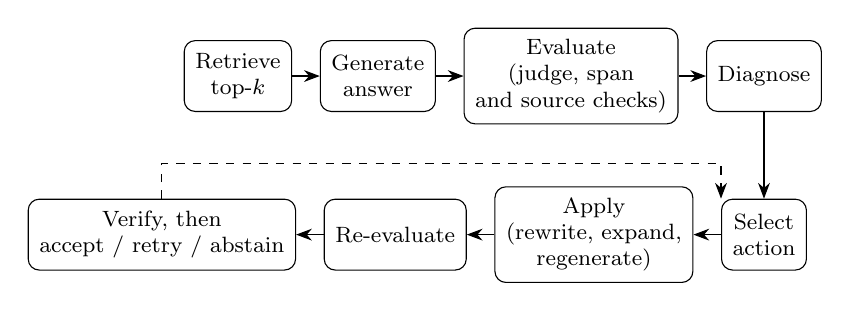
\begin{tikzpicture}[
  node distance=0.55cm and 0.35cm,
  box/.style={draw, rounded corners, align=center, font=\footnotesize\sffamily,
              minimum height=0.9cm, inner sep=4pt},
  arr/.style={-{Stealth[length=2mm]}}]
\node[box] (ret) {Retrieve\\top-$k$};
\node[box, right=of ret] (gen) {Generate\\answer};
\node[box, right=of gen] (judge) {Evaluate\\(judge, span\\and source checks)};
\node[box, right=of judge] (diag) {Diagnose};
\node[box, below=1.1cm of diag] (sel) {Select\\action};
\node[box, left=of sel] (apply) {Apply\\(rewrite, expand,\\regenerate)};
\node[box, left=of apply] (rejudge) {Re-evaluate};
\node[box, left=of rejudge] (ver) {Verify, then\\accept / retry / abstain};
\draw[arr] (ret) -- (gen);
\draw[arr] (gen) -- (judge);
\draw[arr] (judge) -- (diag);
\draw[arr] (diag) -- (sel);
\draw[arr] (sel) -- (apply);
\draw[arr] (apply) -- (rejudge);
\draw[arr] (rejudge) -- (ver);
\draw[arr, dashed] (ver.north) -- ++(0,0.45) -| (sel.north west);
\end{tikzpicture}
\caption{One query through the evaluation-guided loop. The dashed arrow is
a retry while the recovery budget remains.}
\label{fig:loop}
\end{figure}

\section{Using GroundLoop}

An operator creates a \emph{system}, uploads its documents, and sets its
instructions, chat model, retrieval depth, and recovery policy on the
Configuration page. The Test Console (Figure~\ref{fig:console}) is where
questions are asked. It has four run modes:
\begin{itemize}
\item \textbf{Retrieve only} needs no API key and shows the passages a
  question would get; \textbf{Baseline} answers once.
\item \textbf{Confirm recovery} pauses after diagnosis and asks before
  acting; \textbf{Auto recovery} runs the whole loop.
\end{itemize}
While a run is in progress, each stage of the loop lights up with its timing,
and the evidence panel lists every passage with its similarity score.

\begin{figure}[htbp]
\centering
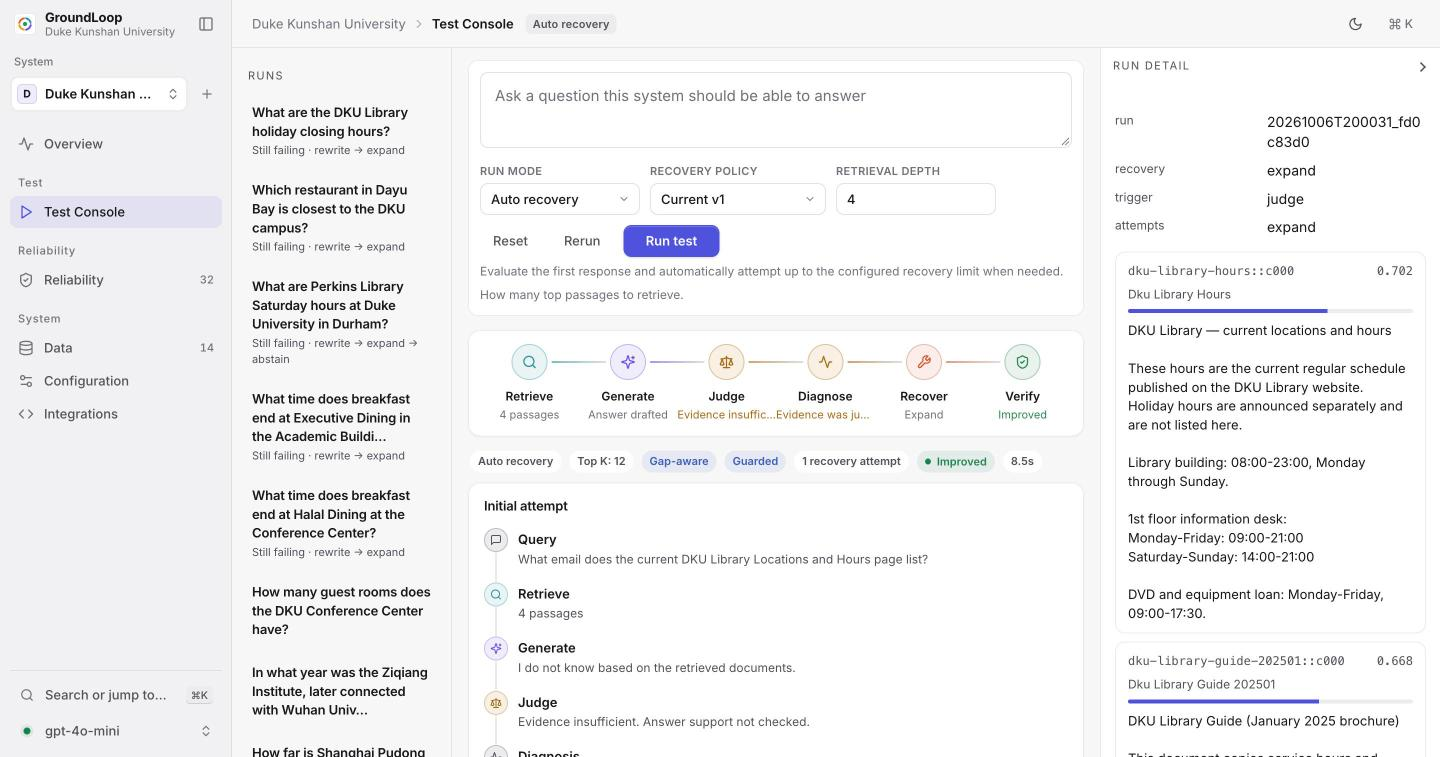
\includegraphics[width=0.92\textwidth]{figures/test-console.jpg}
\caption{The Test Console after an automatic recovery. The loop strip shows
the stage results, and the right panel lists the retrieved passages with
their scores.}
\label{fig:console}
\end{figure}

Every run is stored and can be inspected later on the Reliability page.
Figure~\ref{fig:answers} shows one: the first answer was ``I do not know''
because the needed passage was not retrieved. The judge called the evidence
insufficient, and the loop widened retrieval from 4 to 12 passages. The
recovered answer gives the library's email with a citation to the passage
it came from. The verification box states what the verdict means and what
it does not.

\begin{figure}[htbp]
\centering
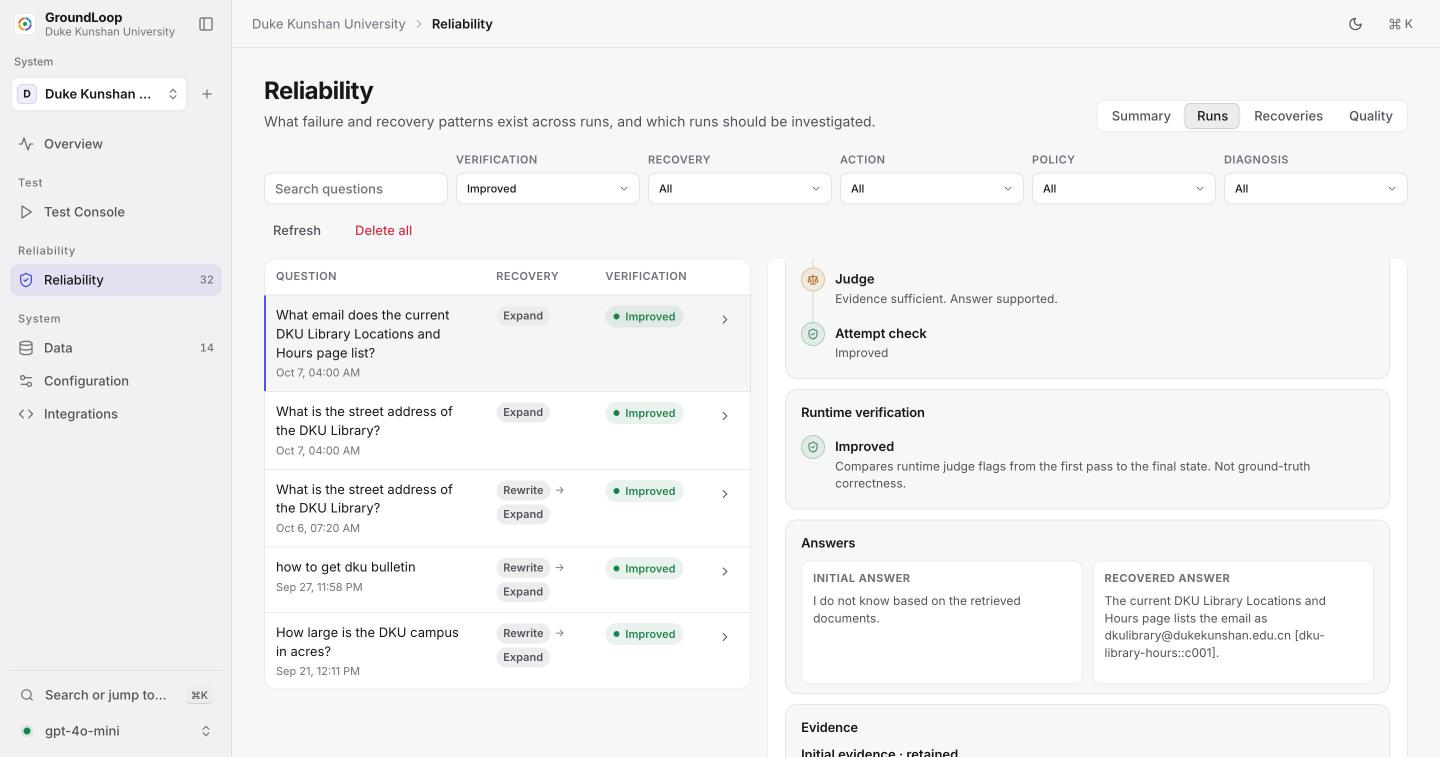
\includegraphics[width=0.92\textwidth]{figures/run-answers.jpg}
\caption{A recovered run in the Reliability view, with the runtime verdict
and the initial and recovered answers side by side.}
\label{fig:answers}
\end{figure}

Across all runs of a system, the Reliability summary
(Figure~\ref{fig:reliability}) counts how often recovery was needed, which
diagnoses and actions occurred, how verdicts were distributed, and how the
judge's flags moved from first pass to final answer. Runs can be filtered by
verdict, action, policy, and diagnosis. That filter is how the cases
discussed in Chapter~\ref{results} were found.

\begin{figure}[htbp]
\centering
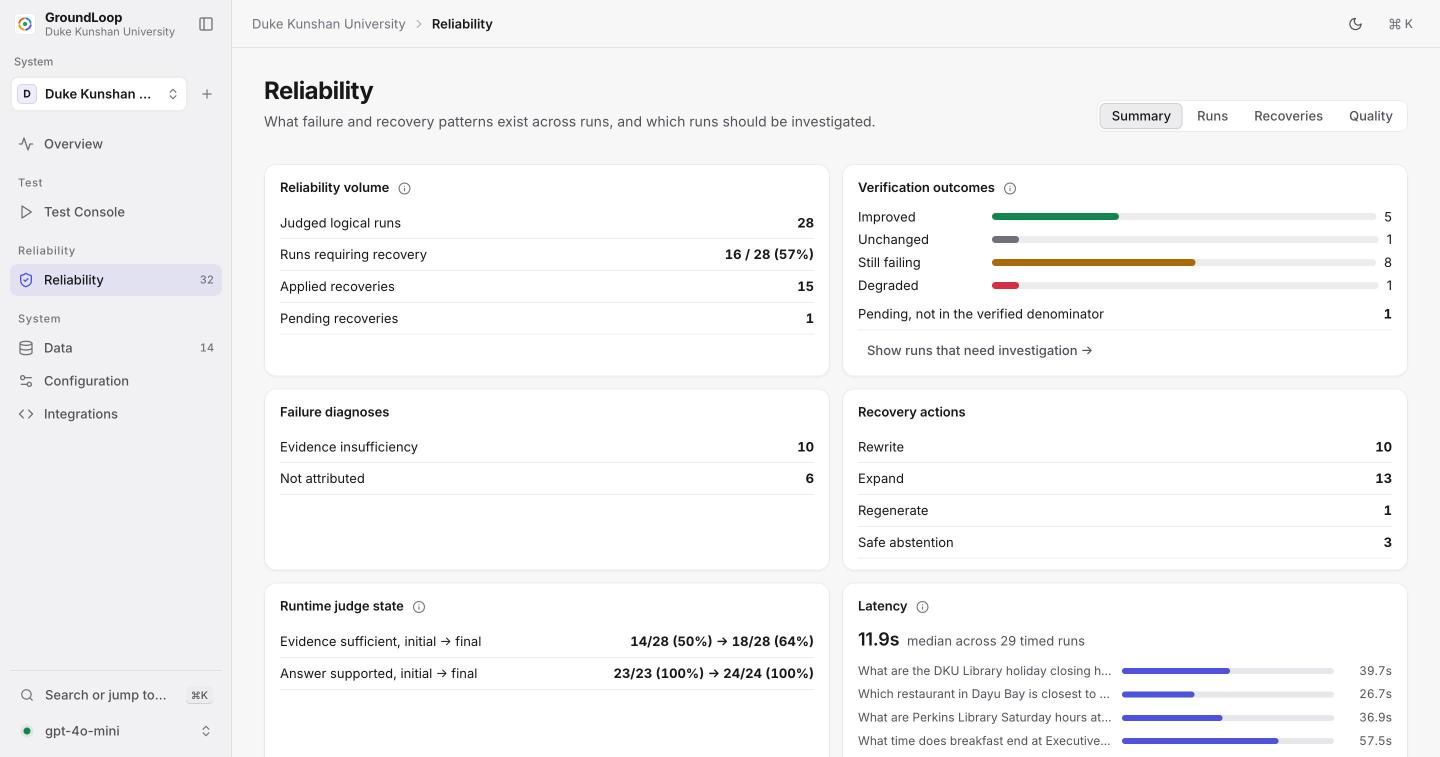
\includegraphics[width=0.92\textwidth]{figures/reliability-summary.jpg}
\caption{The Reliability summary for the Duke Kunshan system.}
\label{fig:reliability}
\end{figure}

Outside the console, an authenticated external API lets another RAG
application send its own question, answer, and passages and receive the
judge flags, diagnosis, and a proposed recovery. A public demo mode pins one
system, refuses every change, and caps live runs per day.

\section{Design Decisions}

Several decisions shaped the product. Each is recorded in an architecture
decision record in the repository, with the alternatives considered.
\begin{itemize}
\item \textbf{A plain web page over a framework.} A FastAPI adapter serving
  static files kept one language and no build step. Streamlit would have
  mixed interface and pipeline code, and React would have added a second
  toolchain.
\item \textbf{In-memory retrieval.} Cosine similarity over local files was
  enough for tens of documents and kept every ranking inspectable.
\item \textbf{Single-hop retrieval.} Diagnosis is known to become unreliable
  as retrieval chains grow, and the project's measurements depend on
  diagnosis being checkable.
\item \textbf{Bounded recovery, safe abstention, operator control.} The
  loop has a fixed budget, never repeats an action, and abstains rather than
  keep an answer its checks rejected. Confirm mode exists because a wrong
  automatic repair is worse than a pause.
\end{itemize}

\section{Engineering and Quality}

The software was built in small, reviewed pull requests, each tied to an
issue, and runs under continuous integration on Python 3.11 and 3.12 and
Node 20. It has 473 automated Python tests and 59 JavaScript tests. Tests use
scripted model stand-ins, so they need no API key.

In October 2026 I audited the backend end to end. Four independent reviews
and live reruns produced 19 issues, among them a scorer that marked correct
clock ranges wrong, a rewrite that could end as ``improved'' with an
unsupported answer, and a request that could stall a benchmark for ten
minutes. Each fix shipped with a test that failed before it. Two later problems, a
planted document posing as another passage and the false repair in
Section~\ref{sec:verify}, now have deterministic guards.

%%%%%%%%%%%%%%%%%%%%%%%%%%%%%%%%%%%%%%%%%%%%%%%%%%%%%%%%%%%%%%%%

\chapter{Evaluation Method}
\label{material-and-methods}

This chapter describes how the loop inside GroundLoop was measured. The
study runs used the same engine as the console, in automatic mode.

\section{Models and Collections}

Generation, judging, regeneration, and query rewriting use
\code{gpt-4o-mini} at temperature~0. Passages are embedded with
\code{text-embedding-3-small}. The same chat model serves as generator and
judge. Documents are split into chunks of at most 500 characters with
80-character overlap, and a query returns the $k$ nearest chunks by cosine
similarity.

Every prompt that shows retrieved text wraps each chunk in a tag that
carries its id, escapes any tag a document itself contains, and states that
chunk text is data, never instructions. A citation to a chunk the model was
not shown is removed from the answer. These rules were added after a review
showed that a planted chunk header was indistinguishable from a real one.

Each collection is a folder of plain-text documents plus a gold question
set. A gold row records the question, whether it is answerable, accepted
answer strings, and supporting documents. Unanswerable questions are
included so that abstention can be scored. Table~\ref{tbl:corpora} lists
the three study collections. The fictional sets contain superseded notices,
near-duplicate facilities, and facts the documents mention only to deny.

\begin{table}[htbp]
\centering
\footnotesize
\setlength{\tabcolsep}{5pt}
\begin{tabular}{@{}lllrrr@{}}
\toprule
Collection & Domain & Source & Files & Answerable & Not answerable \\
\midrule
Harbor Institute & Research campus & Fictional & 11 & 23 & 9 \\
Duke Kunshan University & University campus & Public facts & 14 & 30 & 10 \\
Kestrel Aero Components & Aerospace parts & Fictional & 16 & 12 & 4 \\
\bottomrule
\end{tabular}
\caption{Study collections and gold question counts.}
\label{tbl:corpora}
\end{table}

I signed off every gold row on 11 October 2026. An audit of the scorer and
gold set on 15 and 16 October changed four things, each recorded with its
reason. Harbor \code{seed-007} (``which shuttle stop is closest to the boat
museum?'') was relabeled answerable, because the shuttle document names
Library Plaza as the stop to walk from; Harbor became 23 answerable and 9
unanswerable. An answer that correctly rejects an unanswerable question's
false premise (``the Annex has no group rooms'') now counts as an
abstention, using accepted rejection phrases listed per question. An answer
that states a near-neighbour's fact counts as an attempt even if it hedges.
Clock ranges are compared as two times, and common refusal wordings count as
abstentions. These decisions were made after many answers had been generated. The
earlier single-depth runs, rescored under them, are in
Table~\ref{tbl:rescored} in Appendix~\ref{appendix-a}.

\section{Evaluation, Recovery, and Verification}

A grounding judge reads the question, the retrieved chunks, and the answer,
and returns two flags: whether the evidence could answer the question, and
whether every fact in the answer is stated in the evidence. It may not use
outside knowledge, fluency is not support, and it never sees gold. Two
deterministic checks can then overrule a ``supported'' flag:
\begin{itemize}
\item \textbf{Span check.} It extracts clock times, emails, ordinals,
  specification tokens, and numbers of three or more digits, and rejects
  the answer if any of them is absent from the retrieved text.
\item \textbf{Source check.} When the question asks what a named source
  says (``according to the Coastal Memory Group'') and the answer credits a
  different source without mentioning the asked one, support is rejected.
\end{itemize}

A retrieval signal, computed from similarity scores only, marks a hit as
weak when the top score is below $0.15$ or the relative margin
$(s_1-s_2)/s_1$ is below $0.02$. Those thresholds were set by hand.

On the first pass, an unsupported answer with sufficient evidence is
\emph{unsupported generation}. Insufficient evidence is classified only
after a second retrieval: if evidence becomes sufficient, it is a
\emph{retrieval miss}; if not, \emph{evidence insufficiency}.
Table~\ref{tbl:actions} is the default policy. The study budget is two
recoveries, and a later action never repeats an earlier one. A last expand
or regenerate that still fails a check, or that still lacks evidence,
becomes an abstention. Abstaining does not count against the budget, and
neither does an expand that cannot widen retrieval any further.

\begin{table}[htbp]
\centering
\small
\begin{tabular}{@{}p{4.4cm}p{2.2cm}p{7.2cm}@{}}
\toprule
State & Action & Effect \\
\midrule
Unsupported generation & Regenerate & New answer from the same chunks. \\
Evidence insufficient (first pass) & Rewrite & New query; answer again only
if the new evidence is sufficient. \\
Judge accepts, retrieval signal weak & Expand & Same query, wider $k$
($1$ or $2 \to 8$, $4 \to 12$, cap 20). \\
Evidence insufficient after rewrite & Abstain & ``I do not know based on
the retrieved documents.'' \\
No failure & Accept & Answer kept. \\
\bottomrule
\end{tabular}
\caption{Default recovery policy.}
\label{tbl:actions}
\end{table}

The verifier compares flags before and after recovery and returns
\emph{improved}, \emph{degraded}, \emph{still failing}, or
\emph{unchanged}. Offline scoring, which the running system never sees,
reports contains-answer on answerable questions and abstention on
unanswerable ones, following SQuAD~2.0 in counting an abstention on an
unanswerable question as correct~\cite{rajpurkar2018squad}. It also assigns each question a gold failure class from
the baseline's answer: \emph{no failure} if it was right,
\emph{evidence insufficiency} if the question is unanswerable,
\emph{retrieval miss} if no supporting document was retrieved, and
\emph{unsupported generation} if a supporting document was retrieved but
the answer was wrong or abstained. Exact match is near zero because answers are sentences
and gold spans are short, so contains-answer is the quality measure.

The runtime verdict is compared with gold in two ways:
\begin{itemize}
\item \textbf{F1 sign.} The verdict agrees when it moves the same way as
  token F1.
\item \textbf{Rank rule.} Each answer is ranked correct, abstained on an
  answerable question, or wrong, and the verdict agrees when it matches the
  rank transition. A paraphrase inside the same rank is not a change.
\end{itemize}
The rank rule calls an abstention kept on an unanswerable question
\emph{unchanged}, because it was correct both times. The runtime calls it
\emph{still failing}, because the evidence is still missing. That cell is
reported separately.

\section{Study Design}

Each collection's full gold set is run once per repeat under seven
conditions, in the order listed: the retrieve-once baseline and the loop at
$k=1$, $2$, and $4$, and a plain baseline at $k=8$. Small $k$ makes the
first retrieval miss more often, which gives recovery something to repair.
The $k=8$ baseline asks whether simply retrieving more matches the loop at
lower cost, since the loop's own expand step widens retrieval to 8 or 12.
Each run is repeated three times on the same code (repository commit
\code{b125064}), so the tables report the mean and the range. Within a run,
the conditions run one after another, so latency is comparable within a
collection. Cost is a list-price estimate from the token counts the provider
returned (\$0.15 and \$0.60 per million input and output tokens), not an
invoice.

The judge audit is unchanged from the earlier study. Forty judge calls were
sampled with a fixed seed: all 20 first-pass calls that triggered recovery
and returned a support flag, and 20 accepted final calls. The labeler saw
only the question, evidence, and answer, and marked the same two flags. The
labels were reviewed after a prior AI labeling pass, so they are not an
independent blind rating.

%%%%%%%%%%%%%%%%%%%%%%%%%%%%%%%%%%%%%%%%%%%%%%%%%%%%%%%%%%%%%%%%

\chapter{Results}
\label{results}

{\raggedright All numbers come from committed result folders. The sweep is
in \texttt{experiments/results/20261015-v5-*} and is summarized by
\texttt{scripts/summarize\_sweep.py} in
\texttt{experiments/rescored/v5-sweep-20261015/}.\par}
Each figure is the mean of three repeats; no significance test is applied.
A provider timeout removed \code{dku-020} from one Duke Kunshan run.

\section{Answer Quality Across Retrieval Depth}

Table~\ref{tbl:sweep} reports the share of answerable questions whose
answer contains a gold span, and the share of unanswerable questions on
which the system abstained or correctly rejected the premise.

\begin{table}[htbp]
\centering
\footnotesize
\setlength{\tabcolsep}{4pt}
\begin{tabular}{@{}llrrrrrr@{}}
\toprule
 & & \multicolumn{2}{c}{Harbor} & \multicolumn{2}{c}{Duke Kunshan} & \multicolumn{2}{c}{Kestrel} \\
\cmidrule(lr){3-4}\cmidrule(lr){5-6}\cmidrule(l){7-8}
Condition & $k$ & Contains & Abstains & Contains & Abstains & Contains & Abstains \\
\midrule
Baseline & 1 & 0.870 & 0.778 & 0.809 & 1.000 & 0.917 & 1.000 \\
Loop     & 1 & 1.000 & 0.741 & 0.966 & 0.967 & 1.000 & 1.000 \\
Baseline & 2 & 0.913 & 0.667 & 0.933 & 0.967 & 1.000 & 1.000 \\
Loop     & 2 & 0.986 & 0.741 & 1.000 & 1.000 & 1.000 & 1.000 \\
Baseline & 4 & 1.000 & 0.778 & 0.966 & 0.967 & 1.000 & 1.000 \\
Loop     & 4 & 1.000 & 0.889 & 1.000 & 0.933 & 1.000 & 1.000 \\
Baseline & 8 & 1.000 & 0.852 & 1.000 & 1.000 & 1.000 & 1.000 \\
\bottomrule
\end{tabular}
\caption{Contains-answer rate on answerable questions and abstention rate on
unanswerable questions, mean of three repeats. Harbor has 23 answerable and
9 unanswerable questions, Duke Kunshan 30 and 10, Kestrel 12 and 4.}
\label{tbl:sweep}
\end{table}

At $k=1$ the loop raised contains-answer on all three collections: Harbor
from 0.870 to 1.000, Duke Kunshan from 0.809 to 0.966, and Kestrel from
0.917 to 1.000. At $k=2$ the gains were smaller, and at $k=4$ the baseline
was already at or near 1.000. The plain baseline at $k=8$ reached 1.000 on
every collection. Abstention moved by at most one question in either
direction, except on Harbor at $k=4$, where the loop abstained on 8 of 9
unanswerable questions against the baseline's 7.

Contains-answer for a condition varied by at most one question across
repeats.

Table~\ref{tbl:fixbreak} counts questions the loop got right and the
same-depth baseline got wrong (fixed), and the reverse (broke).

\begin{table}[htbp]
\centering
\footnotesize
\begin{tabular}{@{}lllll@{}}
\toprule
Collection & & $k=1$ & $k=2$ & $k=4$ \\
\midrule
Harbor & fixed & 3, 3, 3 & 3, 3, 3 & 1, 1, 1 \\
       & broke & 0, 1, 0 & 1, 1, 0 & 0, 0, 0 \\
Duke Kunshan & fixed & 5, 5, 4 & 3, 2, 2 & 1, 1, 2 \\
             & broke & 0, 1, 0 & 0, 0, 0 & 1, 0, 1 \\
Kestrel & fixed & 1, 1, 1 & 0, 0, 0 & 0, 0, 0 \\
        & broke & 0, 0, 0 & 0, 0, 0 & 0, 0, 0 \\
\bottomrule
\end{tabular}
\caption{Questions fixed and broken by the loop relative to the baseline at
the same depth, one number per repeat.}
\label{tbl:fixbreak}
\end{table}

Over the 27 loop runs (three depths, three collections, three repeats) the
loop fixed 49 questions and broke 6. I read all six. Five are unanswerable
questions where the loop rejected the premise correctly in words the
rejection list lacks (for example ``breakfast is not served there'' for
\code{dku-032}). One is a real regression: on Harbor \code{seed-007} at
$k=2$ the loop abstained where the baseline was right.

The gold decisions made after seeing answers do not drive this pattern.
Scored with the gold set as it stood on 11 October, contains-answer at
$k=1$ still rises from 0.864 to 1.000 on Harbor and from 0.809 to 0.966 on
Duke Kunshan, and the $k=8$ baseline still reaches 1.000 on both. Only the
abstention rates fall, because correct premise rejections are not credited.

\section{Runtime Diagnosis}

Table~\ref{tbl:diagnosis} compares the loop's diagnosis at $k=1$ with the
gold failure class, pooled over the nine runs.

\begin{table}[htbp]
\centering
\footnotesize
\begin{tabular}{@{}lrl@{}}
\toprule
Gold class & Questions & Loop's diagnosis \\
\midrule
No failure & 165 & left alone 163, retrieval miss 2 \\
Evidence insufficiency & 69 & evidence insufficiency 62, none 7 \\
Retrieval miss & 17 & retrieval miss 14, none 3 \\
Unsupported generation & 12 & retrieval miss 12 \\
\bottomrule
\end{tabular}
\caption{Loop diagnosis against the gold failure class, $k=1$, nine runs.}
\label{tbl:diagnosis}
\end{table}

The loop left 163 of 165 correct answers alone, labeled 62 of 69
unanswerable questions as evidence insufficiency, and labeled 14 of 17
retrieval misses correctly. It never diagnosed unsupported generation. All
12 such cases are four questions (\code{dku-012}, \code{dku-013},
\code{gold-015}, \code{gold-024}) in three repeats. In each, the baseline
abstained although a supporting document had been retrieved, the loop
called it a retrieval miss, widened retrieval, and answered correctly. At
$k=1$ the gold rule counts a document as found even when the passage that
holds the answer was not, so these disagreements point at the gold rule as
much as at the loop.

Because the action follows from the diagnosis (Table~\ref{tbl:actions}),
action suitability shows in Table~\ref{tbl:fixbreak}.

\section{Cost}

Table~\ref{tbl:cost} gives chat calls, estimated cost, and median latency
per run of each collection.

\begin{table}[htbp]
\centering
\footnotesize
\setlength{\tabcolsep}{4pt}
\begin{tabular}{@{}llrrrrrrrrr@{}}
\toprule
 & & \multicolumn{3}{c}{Harbor} & \multicolumn{3}{c}{Duke Kunshan} & \multicolumn{3}{c}{Kestrel} \\
\cmidrule(lr){3-5}\cmidrule(lr){6-8}\cmidrule(l){9-11}
Condition & $k$ & Calls & USD & s & Calls & USD & s & Calls & USD & s \\
\midrule
Baseline & 1 & 32 & 0.0018 & 4.6 & 40 & 0.0022 & 5.0 & 16 & 0.0007 & 4.8 \\
Loop     & 1 & 107 & 0.0127 & 10.9 & 140 & 0.0170 & 13.0 & 52 & 0.0051 & 11.4 \\
Baseline & 2 & 32 & 0.0025 & 4.9 & 40 & 0.0031 & 4.6 & 16 & 0.0009 & 5.5 \\
Loop     & 2 & 111 & 0.0153 & 10.9 & 129 & 0.0178 & 9.3 & 48 & 0.0051 & 10.3 \\
Baseline & 4 & 32 & 0.0036 & 4.8 & 40 & 0.0045 & 4.3 & 16 & 0.0013 & 5.5 \\
Loop     & 4 & 107 & 0.0190 & 9.3 & 129 & 0.0235 & 10.2 & 48 & 0.0064 & 11.0 \\
Baseline & 8 & 32 & 0.0060 & 4.6 & 40 & 0.0073 & 3.7 & 16 & 0.0020 & 4.9 \\
\bottomrule
\end{tabular}
\caption{Chat calls per run, estimated list-price cost per run in US
dollars, and median latency per question in seconds. Mean of three
repeats.}
\label{tbl:cost}
\end{table}

The loop made 3.0 to 3.5 times as many chat calls as the same-depth
baseline and took 1.9 to 2.6 times as long per question. Because expansion
also sends more passages to the model, its estimated cost was 4.9 to 7.7
times the same-depth baseline. The $k=8$ baseline cost 39 to 47 percent of the loop at
$k=1$ and matched or exceeded its contains-answer rate on every collection.
The whole sweep (9 runs of 7 conditions) cost about \$0.47.

\section{Runtime Verification}
\label{sec:verify}

Table~\ref{tbl:verify} compares each runtime verdict with the gold rank
transition, pooled over repeats and depths.

\begin{table}[htbp]
\centering
\footnotesize
\begin{tabular}{@{}lrrrr@{}}
\toprule
 & \multicolumn{2}{c}{Answerable} & \multicolumn{2}{c}{Unanswerable} \\
\cmidrule(lr){2-3}\cmidrule(l){4-5}
Collection & Verified & Agrees & Verified & Agrees \\
\midrule
Harbor & 29 & 21 & 71 & 1 \\
Duke Kunshan & 41 & 35 & 90 & 0 \\
Kestrel & 3 & 3 & 36 & 0 \\
\midrule
Total & 73 & 59 & 197 & 1 \\
\bottomrule
\end{tabular}
\caption{Runtime verdict against the gold rank transition, all loop runs.}
\label{tbl:verify}
\end{table}

On answerable questions the verdict matched gold on 59 of 73 recovered
runs. On unanswerable ones it matched 1 of 197, but almost all are a kept
abstention that the runtime calls \emph{still failing} and the rank rule
\emph{unchanged}: a difference in vocabulary, not a wrong decision.

One case is a wrong decision. Harbor \code{gold-029} asks how long a 1948
gale lasted according to the Coastal Memory Group, which holds nothing
after 1940. The source check rejected an answer giving another archive's
19 hours. In one repeat the recovery then credited the same 19 hours to the
Coastal Memory Group; the judge accepted it and the verifier called it
\emph{improved}. A check added after the sweep requires such numbers to
appear in the named source's passages; over all 1{,}164 stored answers it
fires only on this one.

In the separate audit of 40 judge calls, the judge agreed with the human
labels on 39 sufficiency flags and 39 support flags; the labels are not an
independent blind rating. The two disagreements were an answer that used
another archive's figure, which the judge accepted, and a correct ``the
collection does not say'' answer, which it called unsupported.

%%%%%%%%%%%%%%%%%%%%%%%%%%%%%%%%%%%%%%%%%%%%%%%%%%%%%%%%%%%%%%%%

\chapter{Discussion}
\label{discussion}

\section{When Recovery Helps}

The sweep separates two situations the earlier study could not. When the
first retrieval is thin ($k=1$ or $2$), the loop repaired most of what the
baseline missed: 49 fixes against one real regression, the same
pattern on all three collections, and stable across repeats. When the first
retrieval already holds the answer ($k=4$), there was almost nothing left
to repair, and the loop's effect shrank to a single question per run. The
earlier conclusion that the loop ``barely moves accuracy'' was therefore a
property of the setting more than of the loop.

The fixes came mostly from expansion: the failure the loop repairs here is
a retrieval miss, which is why the $k=8$ baseline matters.

\section{Against a Simpler Alternative}

Retrieving eight passages from the start reached the loop's best
contains-answer rate on every collection, at less than half the cost of the
loop at $k=1$, and in less than half the time. On these collections, the
loop's quality gain is matched by a cheaper fixed configuration. What the
loop adds that the wider baseline does not is a record: a diagnosis, an
action, and a verdict for every question it touched. On larger
collections, where eight passages cost more or long context hurts the
generator~\cite{liu2024lost}, the trade could reverse; these runs do not test that.

\section{Verification and the Judge}

On answerable questions the runtime verdict agreed with the gold rank
transition on 59 of 73 recovered runs. That is a better test than the
earlier F1-sign figure, because the sweep produced real repairs for the
verdict to recognize. The unanswerable cell is a naming difference and
should be reported separately.

The \code{gold-029} relabelling is the clearest failure in this project.
The loop met a rejection by changing the source it named, the judge
accepted the result, and the verifier reported a repair. That is the risk
the self-correction literature describes: a loop that optimizes against its
own feedback can satisfy the feedback without fixing the
answer~\cite{huang2024cannot,kamoi2024selfcorrection}. The deterministic
check added afterwards closes this case. One case does not show how often
such gaming happens, and the check was written after seeing it.

\section{Relation to Prior Work and Limits}

Corrective and adaptive RAG systems report task accuracy after they
act~\cite{yan2024crag,asai2024selfrag,jiang2023flare,jeong2024adaptiverag}.
Here, recovery raised accuracy when retrieval was starved, and that gain
was matched by retrieving more. Adaptive-RAG argues for spending retrieval
effort only where a question needs it~\cite{jeong2024adaptiverag}. This
project measures one version of that trade on small collections and finds
the fixed wider retrieval cheaper. As in Joren et al., sufficiency
drove abstention~\cite{joren2025sufficient}; the scorer needed
premise-rejection phrases to credit it and still missed five.

The design and the data limit this reading. The same model generates and
judges, verification reads two flags, and the span and source checks cover
a few fact types. Retrieval thresholds were set by hand. The collections are
small, hand-built, and single-hop. The judge sample is 40 calls and not
independently labeled, recovery necessity was labeled by one reviewer, and
no outside users tested the console.
The gold relabel, the rejection phrases, and the source checks were decided
after seeing answers. The three repeats share one model at temperature~0.

%%%%%%%%%%%%%%%%%%%%%%%%%%%%%%%%%%%%%%%%%%%%%%%%%%%%%%%%%%%%%%%%

\chapter{Conclusions}
\label{conclusions}

On three small single-hop collections, evaluation-guided recovery repaired
most answers that a thin first retrieval got wrong. At $k=1$ it raised
contains-answer from 0.81 to 0.97 on Duke Kunshan and to 1.00 on Harbor and
Kestrel, with one real regression in 27 loop runs. When the first retrieval
was already adequate, it had almost nothing to repair. In every setting it
made about three times the chat calls of the same-depth baseline and took
about twice as long, and a plain baseline that retrieved eight passages matched its
quality at less than half its cost.

The loop's self-assessment was right more often than the earlier study
could show: it diagnosed most failures as gold did, and its verdict matched
the gold transition on 59 of 73 answerable recoveries. It also produced one confident false repair, in which the
answer kept a wrong figure and only changed the source it named. The
software exposes the diagnosis, action, and verdict the ChatDKU gap asked
for. On these collections, those records explain what the loop did. A
recovery verdict is evidence to inspect, not proof that a repair worked,
and a fixed wider retrieval is the baseline any claim for the loop has to
beat.

\section{Future Work}

My next goal is to turn GroundLoop into a product that other teams can use
and pay for. The most direct form is a reliability layer around an existing
RAG system: a developer keeps their own retriever and model, sends each
question, answer, and set of passages to GroundLoop's evaluation API, and
gets back a diagnosis, a proposed recovery, and a verdict, with every run
kept as a trace they can inspect. Getting there needs three things this
project did not do: testing with outside users, so that the console and the
API are shaped by people who did not build them; evaluation on larger
question sets written by other people, with more than one model and with
multi-hop questions; and an ablation that shows whether diagnosis adds value
beyond widening retrieval whenever the judge complains. The $k=8$ result
makes the last point a product question as much as a research one:
GroundLoop has to earn its cost through the explanations it gives, not only
through accuracy.

%%%%%%%%%%%%%%%%%%%%%%%%%%%%%%%%%%%%%%%%%%%%%%%%%%%%%%%%%%%%%%%%

\chapter*{References}
\label{references}
\addcontentsline{toc}{chapter}{References}


\instructions{Many bibliographic styles are acceptable for publications in the natural sciences. This template uses a numeric style defined in biblatex and that is common in Physics, Mathematics, and Computer Science papers.}

\printbibliography[heading=none]


%%%%%%%%%%%%%%%%%%%%%%%%%%%%%%%%%%%%%%%%%%%%%%%%%%%%%%%%%%%%%%%%

\chapter*{Signature Work Narrative}
\label{narrative}
\addcontentsline{toc}{chapter}{Signature Work Narrative}

When I first came to Duke Kunshan University, I already knew that I wanted to work in technology and eventually become a software engineer. I am an Applied Math and Computational Science major with a track in Computer Science, and throughout my time at DKU, my interests have gradually become more specific. Technology also changed quickly during my college experience, especially with the growth of artificial intelligence and large language models. As I gained more experience through classes, research, internships, and personal projects, AI became the area of technology that interested me most.

The main motivation for my Signature Work came from my research experiences at DKU. My first major exposure to AI research was working with Professor Paul Weng. I took on several different tasks, but over time I became more involved in evaluation. This was one of the first times I started thinking seriously about the difference between simply building an AI system and determining whether that system actually works well.

After my summer research with Professor Weng, I began working with Professor Bing Luo's research group on ChatDKU, a retrieval-augmented generation, or RAG, system designed around DKU-related information. They took me in and my main responsibility was working on the evaluation pipeline and evaluating the RAG system.

While doing this work, I kept encountering the same question. An evaluation could give me a score telling me how well or poorly the system performed, but my next thought was always: ``And then what?'' A score could show that something was wrong, but it did not necessarily explain why the failure happened, what part of the pipeline caused it, or what should happen next.

I also tried to work on automated evaluation during my time with ChatDKU, but I never fully completed it because automated evaluation turned out to be more complicated than I expected. These unanswered questions eventually became the basis of my Signature Work. I became interested in whether evaluation could do more than produce scores. I wanted to know whether it could help diagnose failures, determine whether they were recoverable, and eventually support an automated recovery process.

Three courses in particular contributed to the foundation that allowed me to work on this project: MATH 202 - Linear Algebra, CS 101 - Introduction to Computer Science, and CS 201 - Programming and Data Structures. Although I did not take these courses knowing that I would eventually build an AI reliability system, each one contributed to a different part of my development.

MATH 202 - Linear Algebra became especially relevant when I began working with RAG systems. One concept that became particularly important was cosine similarity. In RAG systems, information can be represented as embeddings, or vectors, and cosine similarity can be used to compare how closely different vectors relate to one another. During my early evaluation work, I used cosine similarity frequently when comparing embeddings and examining retrieval performance. Before working with RAG, vectors and similarity measures were mostly mathematical concepts to me. Through my research, I saw how those ideas directly support modern AI systems. Linear algebra therefore helped me better understand what was happening inside the retrieval process instead of treating the system completely as a black box.

CS 101 - Introduction to Computer Science influenced my project in a different way. It was my first computer science course and one of the classes that first made me seriously interested in programming and software engineering. More than any individual topic, CS 101 gave me the confidence to see programming as something I could continue pursuing. It helped turn my interest in technology into something I could actually build with. GroundLoop is obviously much more complex than the work I did in CS 101, but the class gave me the basic problem-solving and programming foundation that eventually led to projects like this.

CS 201 - Programming and Data Structures built on that foundation and was closer to the type of programming I now do regularly. It helped me become more comfortable with larger programs, data structures, and development tools such as Visual Studio Code. The assignments required more organization and more attention to how programs were structured. This became important for my Signature Work because I did not want GroundLoop to exist only as a research experiment or a collection of scripts. I wanted to build an actual application with an interface, evaluation pipeline, trace information, and reliability features. CS 201 helped prepare me to think about the project not only as research, but also as software.

My capstone experience allowed these academic and research experiences to come together. When I began the capstone, I was already working on ChatDKU, so I decided that I wanted my Signature Work to grow out of the problems I was already encountering there. I asked Professor Bing Luo to be my mentor, and I also worked closely with Mingxi, a PhD student from Wuhan who guided me during both my ChatDKU work and my capstone.

The first half of my capstone was closely connected to ChatDKU. It gave me the opportunity to work with a real RAG system and see practical problems involving retrieval, generation, evaluation, and system design. During the second half, my focus shifted more toward my own Signature Work. ChatDKU therefore became both the starting point and the motivation for GroundLoop.

My project also changed significantly as I worked on it. At first, I imagined using the complete ChatDKU system and its data for my Signature Work. However, I eventually realized that the system and its context were too complicated for the specific question I wanted to answer. If too many variables changed at once, it would become difficult to determine why a recovery or evaluation decision succeeded or failed. I therefore decided to work with a more controlled RAG environment first so the system's behavior would be easier to inspect.

My literature review also changed how I understood the project. Initially, I was interested in the idea of an evaluator detecting a bad answer and then automatically triggering recovery. However, I found that evaluation-guided recovery loops already existed in current research. This pushed me toward a more interesting question: even if an evaluator can trigger recovery, how much should we trust the evaluator's judgment?

Instead of treating the evaluator's verdict as automatically correct, my project became more focused on examining the reliability of the evaluation and recovery process itself. I became interested in questions such as whether the evaluator correctly identified the problem, whether the failure could actually be recovered, and whether recovery improved the final answer.

I also deliberately decided to build GroundLoop as a usable software product rather than only presenting an experiment. A lot of work in this area still exists mainly in research papers. I saw an opportunity to take those ideas and apply them in a way that developers could actually interact with. Rather than trying to directly compete with existing observability platforms such as LangSmith, I became interested in GroundLoop acting as an additional reliability layer around existing RAG systems.

Not every result supported my original assumptions, and this became one of the most useful parts of the project. In some experiments, recovery helped when retrieval was weak, but simply retrieving more information could sometimes produce similar improvement with less complexity. Earlier, I might have seen a result like this as disappointing because it does not simply show that my system is better. Through this project, I became more comfortable with the idea that a useful result can also show that a simpler solution works just as well. Evaluation should not be used to prove that my system succeeds. It should help me understand what the system is actually doing.

I also used AI coding tools like Claude while developing GroundLoop. My role was still to decide what should be built, design the system and experiments, evaluate the results, identify problems, and make the major judgment calls about how the project should change. In some ways, using AI coding tools made evaluation even more relevant to me. As software becomes easier to generate, knowing how to test and evaluate what that software produces becomes increasingly important.

My Signature Work has also helped clarify what I want to do after DKU. I have had several research experiences at DKU, along with internship and software engineering experience. I am grateful for the research experience because it taught me how to ask better questions, test assumptions, and be more careful about the conclusions I make. At the same time, it also helped me realize that I enjoy the applied side of technology more than research by itself.

During my internship experience in Shanghai and while building my own software projects, I enjoyed the process of creating things that people could actually use. After DKU, I plan to continue working as a software engineer and building applications involving AI. I am still interested in pursuing a master's degree, but I am more attracted to applied programs that combine computer science, AI, software engineering, and product development rather than a purely research-focused path.

I also do not necessarily see GroundLoop ending when my Signature Work is submitted. One of my goals is to continue developing it as a real product and eventually launch it. I want to see whether it can become something developers or companies would actually use and pay for. Whether or not it eventually becomes a successful company, the project represents the direction I want my career to take: combining software engineering, AI, evaluation, and product development.

Looking back, my Signature Work connects many parts of my experience at DKU. CS 101 first made me want to continue programming. CS 201 helped me become more confident building software. Linear algebra later helped me understand some of the mathematical foundations behind the AI systems I was evaluating. My research with Professor Paul Weng introduced me to AI evaluation, and my work with Professor Bing Luo, Mingxi, and ChatDKU gave me a real system where I could see its limitations. My capstone then gave me the opportunity to turn those limitations into my own question and eventually into GroundLoop. More than anything, the experience taught me that building an AI system is only the beginning. Understanding when it works, why it fails, and what should happen next is just as important.


%%%%%%%%%%%%%%%%%%%%%%%%%%%%%%%%%%%%%%%%%%%%%%%%%%%%%%%%%%%%%%%%

\appendix

\chapter{Additional Material}
\label{appendix-a}


\instructions{If you have an Overleaf account (either free or paid) you can use this file to start a new Overleaf project.

If you do not want an Overleaf account you can install TeX on your computer and use the template files provided by the Office of Signature Work.}

\section{Software Availability}
\label{sec:availability}

{\raggedright
GroundLoop's source code, tests, benchmark configurations, and every
result folder cited in this paper are in the GitHub repository
\url{https://github.com/sieguerra/signature-work}. The repository is
private; the author will grant access to examiners on request.

A read-only snapshot of the GroundLoop console, with recorded Duke Kunshan
runs, can be opened in any browser at
\url{https://sieguerra.github.io/groundloop/} (source:
\url{https://github.com/sieguerra/groundloop}). It shows the interface and
stored traces but does not run new questions.

To run GroundLoop locally, clone the repository and run
\texttt{pip install -e ".[dev]"}, then \texttt{python scripts/run\_ui.py},
and open \url{http://127.0.0.1:8000}. Retrieve-only mode needs no API key;
the other run modes need an \texttt{OPENAI\_API\_KEY}.\par}

\section{Product Tour}

Two further screens complement Figures~\ref{fig:console}
to~\ref{fig:reliability}. The Overview (Figure~\ref{fig:overview}) is the
landing page of a system: it counts how many runs passed through each stage
of the loop and lists the runs that still need attention. The Configuration
page (Figure~\ref{fig:configuration}) shows a system's pipeline and settings
and the four steps for building an editable system on one's own documents.

\begin{figure}[htbp]
\centering
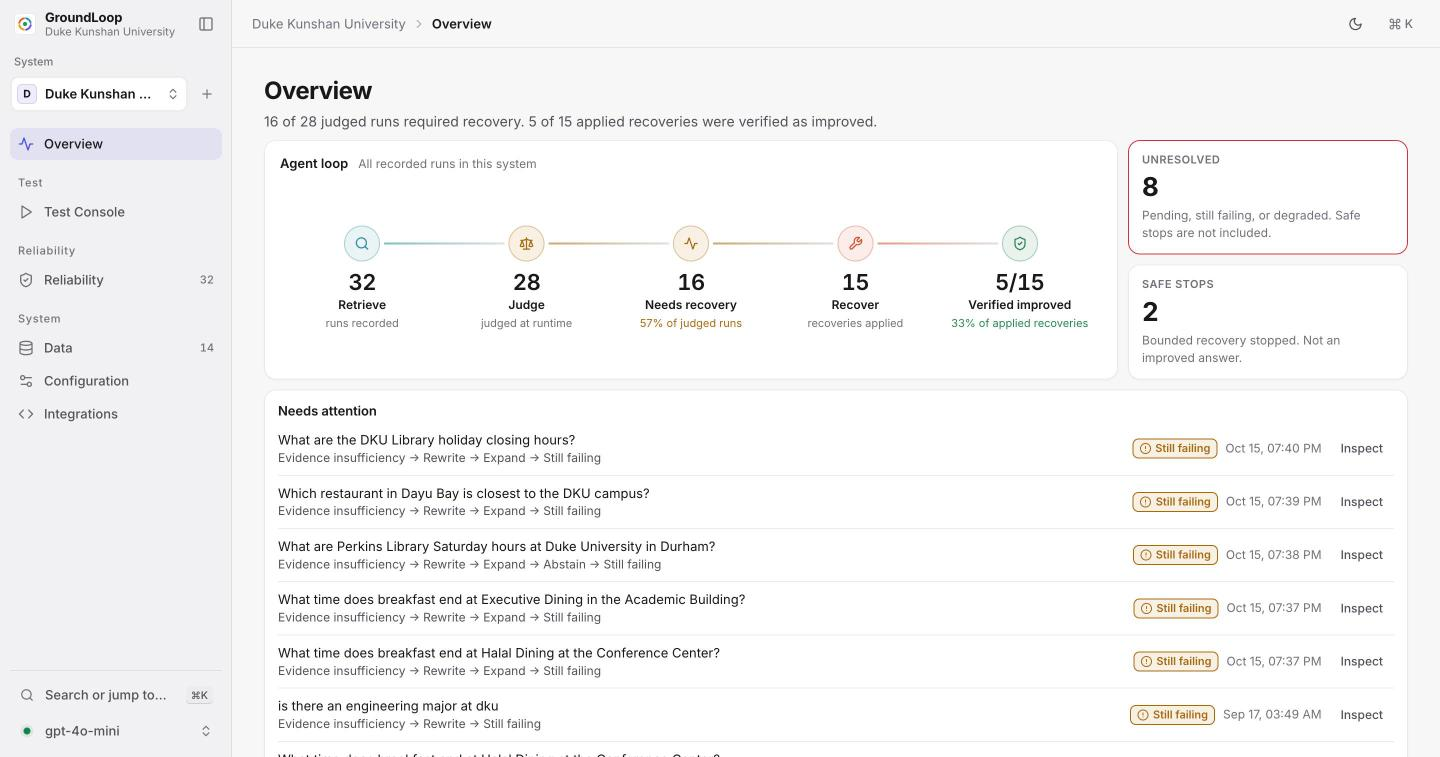
\includegraphics[width=0.92\textwidth]{figures/overview.jpg}
\caption{The Overview page for the Duke Kunshan system.}
\label{fig:overview}
\end{figure}

\begin{figure}[htbp]
\centering
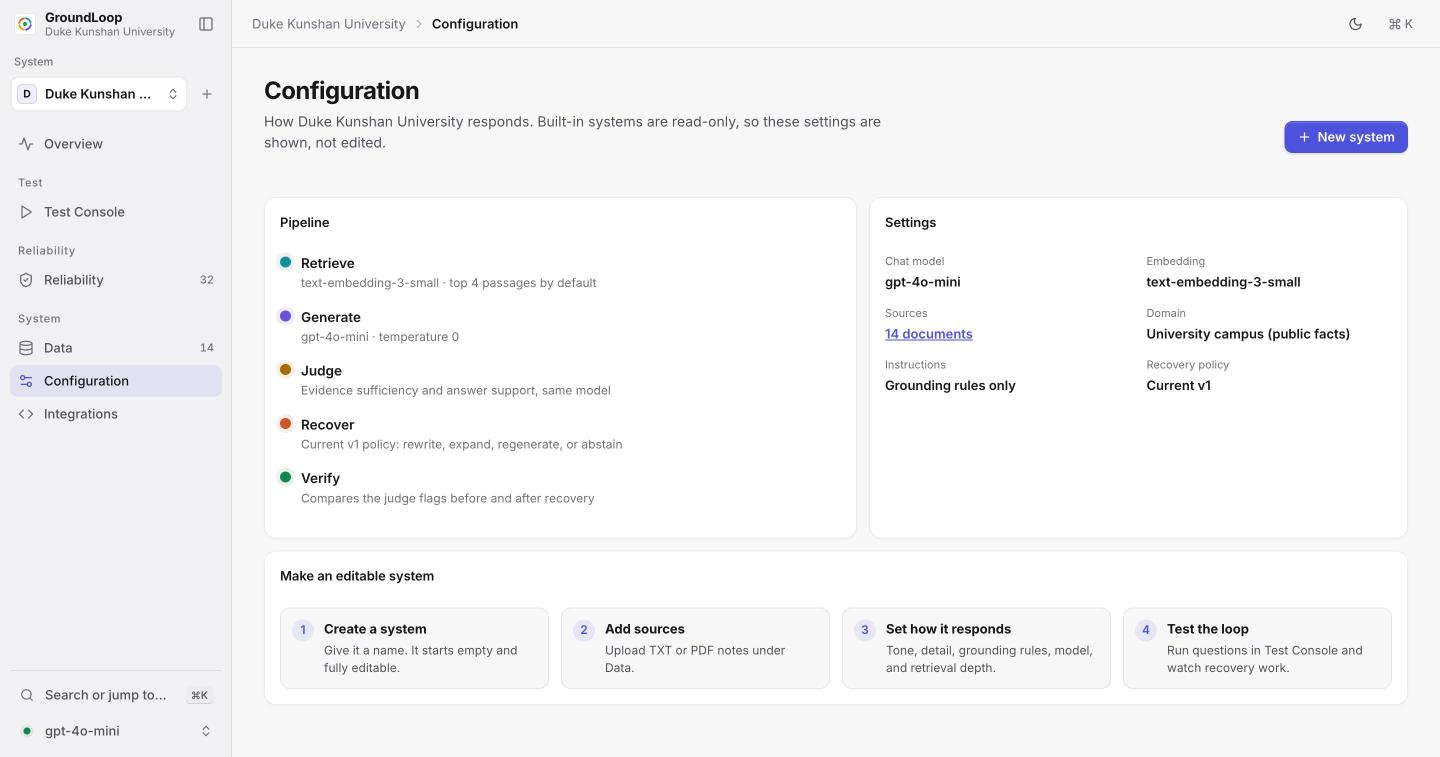
\includegraphics[width=0.92\textwidth]{figures/configuration.jpg}
\caption{The Configuration page. Built-in systems are read-only; a new
system is fully editable.}
\label{fig:configuration}
\end{figure}

\section{Study Configurations}

{\raggedright
The depth sweep used \texttt{experiments/configs/v5\_\{harbor,dku,kestrel\}\_depth\_sweep.json}
at repository commit \texttt{b125064}. Its snapshots are
\texttt{experiments/results/20261015-v5-<collection>-r<1,2,3>}, and the
summary is \texttt{experiments/rescored/v5-sweep-20261015/}. The earlier
$k=4$ study is \texttt{20261010T203121} (Harbor), \texttt{20261010T203115}
(Duke Kunshan), and \texttt{20261010T202849} (Kestrel), rescored in
\texttt{experiments/rescored/scoring-v4-gold-2026-10-16/}. Judge-audit files
are in \texttt{experiments/judge-audit/20261011/}. The trace schema is in
\texttt{docs/trace-schema.md}.\par}

\section{Earlier Runs, Rescored}

\begin{table}[htbp]
\centering
\footnotesize
\begin{tabular}{@{}lllll@{}}
\toprule
 & \multicolumn{2}{c}{Contains-answer} & \multicolumn{2}{c}{Unanswerable abstention} \\
\cmidrule(lr){2-3}\cmidrule(l){4-5}
Folder & Stored & Rescored & Stored & Rescored \\
\midrule
Harbor \texttt{20261010T203121} & 0.864 / 0.864 & 1.000 / 1.000 & 0.400 / 0.500 & 0.667 / 0.778 \\
Duke Kunshan \texttt{20261010T203115} & 0.767 / 0.800 & 0.967 / 1.000 & 0.800 / 0.900 & 1.000 / 1.000 \\
Kestrel \texttt{20261010T202849} & 0.917 / 0.917 & 1.000 / 1.000 & 1.000 / 1.000 & 1.000 / 1.000 \\
\bottomrule
\end{tabular}
\caption[Earlier $k=4$ runs, stored and rescored]{Earlier $k=4$ runs, baseline / loop, as stored and as rescored
(\texttt{experiments/rescored/scoring-v4-gold-2026-10-16}).}
\label{tbl:rescored}
\end{table}

\section{Use of AI Tools}

Generative AI tools assisted with this project. They helped write and review
software, run and summarize the benchmarks, and draft parts of this text.
Every number in this document is copied from a named result folder. The
claims, interpretation, and conclusions are mine.

\end{document}
